\boxde
\BTTN
\begin{ex}%[2D1N3-1]Câu 2
 Đường thẳng $x = a$ là một đường tiệm cận đứng của
 đồ thị hàm số $ y = f (x)$ nếu điều kiện sau thoả mãn
 \choice
 {$\displaystyle\lim_{x\to +\infty }f(x)=a$}
 {\True $\displaystyle\lim_{x\to a^-}f(x)=+\infty $}
 {$\displaystyle\lim_{x\to -\infty }f(x)=a$}
 {$\displaystyle\lim_{x\to a^-}f(x)=a $}
 \loigiai{ Đường thẳng $x = a$ được gọi là một đường tiệm cận đứng (hay tiệm cận đứng) của đồ thị hàm số $ y = f (x)$ nếu ít nhất một trong các điều kiện sau thoả mãn: \\$\displaystyle\lim_{x\to a^+}f(x)=+\infty $, $\displaystyle\lim_{x\to a^+}f(x)=-\infty $, $\displaystyle\lim_{x\to a^-}f(x)=-\infty $, $\displaystyle\lim_{x\to a^-}f(x)=+\infty $.}
\end{ex}
\begin{ex}%[2D1N3-1]Câu 4
 Đường thẳng $y = ax + b$ ($a \neq 0$) được gọi là đường tiệm cận xiên của đồ thị hàm số $y = f(x)$ nếu
 \choice
 {\True $\displaystyle\lim_{x\to -\infty }\big(f(x)-ax-b\big)=0$ hoặc $\displaystyle\lim_{x\to +\infty }\big(f(x)-ax-b\big)=0$}
 {$\displaystyle\lim_{x\to -\infty }\big(f(x)-ax+b\big)=0$ hoặc $\displaystyle\lim_{x\to +\infty }\big(f(x)-ax+b\big)=0$}
 {$\displaystyle\lim_{x\to 0 }\big(f(x)-ax+b\big)=+\infty$ hoặc $\displaystyle\lim_{x\to 0 }\big(f(x)-ax+b\big)=+\infty$}
 {$\displaystyle\lim_{x\to 0 }\big(f(x)-ax-b\big)=-\infty$ hoặc $\displaystyle\lim_{x\to 0 }\big(f(x)-ax-b\big)=-\infty$}
 \loigiai{Đường thẳng $y = ax + b, a \neq 0$, được gọi là đường tiệm cận xiên (hay tiệm cận xiên) của đồ thị hàm số $y = f(x)$ nếu\\ $\displaystyle\lim_{x\to -\infty }[f(x)-(ax+b)]=\displaystyle\lim_{x\to -\infty }(f(x)-ax-b)=0$ hoặc\\ $\displaystyle\lim_{x\to +\infty }[f(x)-(ax+b)]=\displaystyle\lim_{x\to +\infty }(f(x)-ax-b)=0$.
 }
\end{ex}
\begin{ex}
 Tiệm cận ngang của đồ thị hàm số $ y=\dfrac{2x-1}{x+1} $ là đường thẳng
 \choice
 {$y=-1$}
 {$ x=-1 $}
 {\True $ y=2 $}
 {$ x=2 $}
 \loigiai
 {
 Ta có $ \lim\limits_{x\to \pm\infty}y=2$ suy ra đường thẳng $ y=2 $ là tiệm cận ngang của đồ thị hàm số $ y=\dfrac{2x-1}{x+1} $.
 }
\end{ex}
\begin{ex}
 Tiệm cận ngang của đồ thị hàm số $y=\dfrac{1}{2x-3}$ là đường thẳng
 \choice
 {$y=\dfrac{3}{2}$}
 {$x=\dfrac{3}{2}$}
 {\True $y=0$}
 {$y=\dfrac{1}{2}$}
 \loigiai{
 Vì $\lim\limits_{x\to -\infty} \dfrac{1}{2x-3}=\lim\limits_{x\to +\infty} \dfrac{1}{2x-3}=0$ nên đồ thị hàm số có tiệm cận ngang $y=0$.
 }
\end{ex}
\begin{ex}
 Đồ thị hàm số $f(x)=\dfrac{2x-3}{x+1}$ có đường tiệm cận đứng là
 \choice
 {$y=2$}
 {\True $x=-1$}
 {$y=-1$}
 {$x=2$}
 \loigiai{
 Ta có $\displaystyle \lim_{x \to (-1)^-}f(x)=\displaystyle \lim_{x \to (-1)^-}\dfrac{2x-3}{x+1}=+\infty $; $\displaystyle \lim_{x \to (-1)^+}f(x)=\displaystyle \lim_{x \to (-1)^+}\dfrac{2x-3}{x+1}=-\infty$ nên đường thẳng $x=-1$ là đường tiệm cận đứng của đồ thị hàm số.}
\end{ex}
\begin{ex}
 Hàm số nào sau đây có đồ thị nhận đường thẳng $x=2$ là đường tiệm cận đứng?
 \choice
 {$y=\dfrac{2}{x+2}$}
 {\True $y=\dfrac{5x}{2-x}$}
 {$y=\dfrac{1}{x+1}$}
 {$y=x-2+\dfrac{1}{x+1}$}
 \loigiai{
 Ta có $\lim\limits_{x\to 2^+} \dfrac{5x}{2-x}=-\infty $ và $\lim\limits_{x\to 2^-} \dfrac{5x}{2-x}=+\infty $ nên đồ thị hàm số $y=\dfrac{5x}{2-x}$ nhận $x=2$ làm tiệm cận đứng.}
\end{ex}
\begin{ex}%[2D1V3-1]Câu 12
 Đồ thị của hàm số nào sau đây có giao điểm của hai đường tiệm cận thuộc đường thẳng $y=x$?
 \choice
 {$y=\dfrac{2x-1}{x+3}$}
 {\True$y=\dfrac{x+4}{x-1}$}
 {$y=\dfrac{2x+1}{x+2}$}
 {$\dfrac{1}{x+3}$}
 \loigiai{
 Đáp án $y=\dfrac{2x-1}{x+3}$ có giao hai đường tiệm tiệm cận là $(-3;2)\notin d$\\
 Đáp án $y=\dfrac{x+4}{x-1}$ có giao hai đường tiệm cận là $(1;1)\in d$\\
 Đáp án $y=\dfrac{2x+1}{x+2}$ có giao hai đường tiệm cận là $(-2;2)\notin d$\\
 Đáp án $\dfrac{1}{x+3}$ có giao hai đường tiệm cận là $(-3;0)\notin d$\\
 }
\end{ex}
\begin{ex}%[2D1N3-1]Câu 6
 Đồ thị hàm số $y=\dfrac{x-2}{x^{2}-4}$ có mấy đường tiệm cận?
 \choice
 {$3$}
 {$1$}
 {\True$2$}
 {$0$}
 \loigiai{ Hàm số $y=\dfrac{x-2}{x^{2}-4}=\dfrac{x-2}{(x-2)(x+2)}=\dfrac{1}{x+2}$.\\
 $\heva{&\displaystyle\lim_{x\to +\infty }\dfrac{1}{x+2}=0\\&
 \displaystyle\lim_{x\to -\infty }\dfrac{1}{x+2}=0.}$\\
 Nên $y=0$ là đường tiệm cận ngang của hàm số, hàm số có tiệm cận ngang thì không có tiệm cận xiên.\\
 $\heva{&\displaystyle\lim_{x\to -2^- }\dfrac{1}{x+2}= - \infty \\&
 \displaystyle\lim_{x\to -2^+ }\dfrac{1}{x+2}= + \infty.}$\\
 Nên $x=-2$ là đường tiệm cận đứng của hàm số.\\
 Vậy hàm số có hai đường tiệm cận.
 }
\end{ex}
\begin{ex}
 Tiệm cận xiên của đồ thị hàm số $y=\dfrac{x^2+x-1}{x}$ có phương trình là
 \choice
 {$y=x-1$}
 {$y=x-2$}
 {$y=x-3$}
 {\True$y=x+1$}
 \loigiai{
 Ta có $y=\dfrac{x^2+x-1}{x}=x+1-\dfrac{1}{x}$.\\
 Xét $$\displaystyle\lim_{x\to \pm \infty }\big(y-(x+1)\big)=\displaystyle\lim_{x\to \pm \infty }\dfrac{-1}{x}=0$$
 Vậy đường tiệm cận xiên cần tìm của hàm số $f(x)$ có phương trình $y=x+1$.}
\end{ex}
\begin{ex}
 Tiệm cận xiên của đồ thị hàm số $y=\dfrac{2x^2-3x+4}{x-1}$ có phương trình là
 \choice
 {$y=x-1$}
 {\True $y=2x-1$}
 {$y=2x+1$}
 {$y=x+1$}
 \loigiai{
 Ta có $y=\dfrac{2x^2-3x+4}{x-1}=2x-1+\dfrac{3}{x-1}$. Suy ra $y=2x-1$ là đường tiệm cận xiên của đồ thị hàm số.
 }
\end{ex}
\begin{ex}
 Cho hàm số $y=f(x)$ xác định $ \mathbb{R} \setminus \left\lbrace 0\right\rbrace $, liên tục trên mỗi khoảng xác định và có bảng biến thiên như sau.\\
 \begin{center}
 
\begin{tikzpicture}[>=stealth,font=\footnotesize,scale=1]
 \tikzset{double style/.append style = {draw=\tkzTabDefaultWritingColor,double=\tkzTabDefaultBackgroundColor,double distance=2pt}}
 \tkzTabInit[nocadre=false,lgt=1.2,espcl=2.5,deltacl=0.6]
 {$x$ /0.6,$y'$ /0.6,$y$ /2}
 {$-\infty$,$0$,$ 1 $,$+\infty$}
 \tkzTabLine{,-,d,+,$ 0 $,- }
 \tkzTabVar{+/ $+\infty$,-D- /$-1$/$-\infty$,+/$2$,-/$ -\infty $}
 \end{tikzpicture}
 \end{center}
 Chọn khẳng định đúng
 \choice
 {Đồ thị hàm số có hai tiệm cận ngang}
 {\True Đồ thị hàm số có đúng một tiệm cận đứng}
 {Đồ thị hàm số không có tiệm cận đứng và tiệm cận ngang}
 {Đồ thị hàm số có đúng một tiệm cận ngang}
 \loigiai
 {
 Dựa vào bảng biến thiên ta thấy
 $ \lim\limits_{x \to + \infty} f(x)=+\infty$; $ \lim\limits_{x \to -\infty}f(x)=-\infty$; $ \lim\limits_{x \to 0^+}f(x)=-\infty$.\\
 Suy ra đồ thị hàm số có đúng một tiệm cận đứng.
 }
\end{ex}
\begin{ex}%[2D1N3-1]Câu 5
 \immini{Cho hàm số $y=f(x)$ có đồ thị như hình bên dưới. Khẳng định nào sau đây là khẳng định đúng?
 \choice
 {Đồ thị hàm số chỉ có 2 đường tiệm cận đứng $x=-1$ và $x=1$}
 {\True Đồ thị hàm số có 3 đường tiệm cận}
 {Đồ thị hàm số có 4 đường tiệm cận}
 {Đồ thị hàm số có 2 đường tiệm cận đứng và 1 đường tiệm cận xiên}}{
 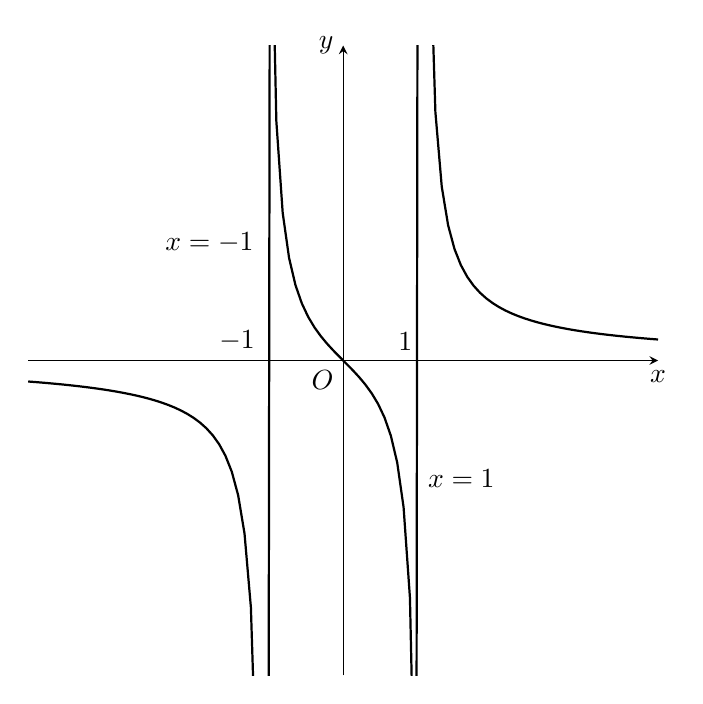
\begin{tikzpicture}[>=stealth]
 \draw[->] (-4,0) --(4,0);
 \draw[->](0,-4)--(0,4);
 \draw (0,0) node[below left]{$O$};
 \draw (4,0) node[below]{$x$};
 \draw (0,4) node[left]{$y$};
 \draw (1,0) node[above left]{$1$};
 \draw (-1,0) node[above left]{$-1$};
 \clip (-4,-4) rectangle(4,4);
 \draw[thick,samples=100] plot[domain=-4:4]
 (\x,{(\x)/((\x)^(2)-1)});
 \draw (-1.7,1.5) node
 {$x=-1$};
 \draw (1.5,-1.5) node
 {$x=1$};
 \end{tikzpicture}}
 \loigiai{ Đồ thị hàm số có 2 đường tiệm cận đứng $x=-1$ và $x=1$ và một đường tiệm cận ngang $y=0$, hàm số không có đường tiệm cận xiên.}
\end{ex}
\begin{ex}
 Biết rằng đồ thị hàm số $ y=\dfrac{ax+1}{bx-2}$ có tiệm cận đứng là $x=2$ và tiệm cận ngang là $y=3$. Giá trị của $a+b$ bằng
 \choice
 {$0$}
 {\True $4$}
 {$5$}
 {$1$}
 \loigiai{
 Điều kiện để đồ thị hàm số $ y=\dfrac{ax+1}{bx-2}$ có tiệm cận đứng và tiệm cận ngang là $-2a-b\ne 0$. \quad$(*)$\\
 $b\ne 0$ vì nếu $ b=0$, đồ thị hàm số $ y=\dfrac{ax+1}{-2}$ không có tiệm cận.\\
 Tập xác định của hàm số $y=\dfrac{ax+1}{bx-2}$ là $\mathscr{D}=\left(-\infty;\dfrac{2}{b}\right)\cup\left(\dfrac{2}{b};+\infty\right)$.\\
 $\lim\limits_{x\to\pm\infty}\dfrac{ax+1}{bx-2}=\dfrac{a}{b}\Rightarrow y=\dfrac{a}{b}$ là đường tiệm cận ngang của đồ thị hàm số.\\
 Theo giả thiết ta có $\dfrac{a}{b}=3\Leftrightarrow a=3b$.\\
 Đồ thị hàm số $y=\dfrac{ax+1}{bx-2}$ có $ x=\dfrac{2}{b}$ là đường tiệm cận đứng.\\
 Theo giả thiết ta có $\dfrac{2}{b}=2\Leftrightarrow b=1\Rightarrow a=3$ (thỏa mãn điều kiện $(*)$).\\
 Vậy $a+b=4$.
 }
\end{ex}
\begin{ex}
 Tìm tất cả giá trị của tham số $m$ để đường tiệm cận xiên của đồ thị hàm số $y=2mx+3-\dfrac{4}{x+1}$ đi qua điểm $M(1;7)$.
 \choice
 {$m=1$}
 {$m=3$}
 {\True $m=2$}
 {$m=-2$}
 \loigiai{
 Xét $\displaystyle\lim_{x\to \pm \infty }\left( y-\left( 2mx+3\right) \right) =\displaystyle\lim_{x\to \pm \infty }\dfrac{-4}{x+1}=0$.\\
 Vậy đường tiệm cận xiên có phương trình $y=2mx+3$.\\
 Đường thẳng này qua điểm $M(1;7)$, suy ra $2m \cdot 1 ++3=7 \Leftrightarrow m=2$.
 }
\end{ex}
\begin{ex}
 Tại một công ty sản xuất đồ chơi A, công ty phải chi 50000 USD để thiết lập dây chuyền sản xuất ban đầu. Sau đó, cứ sản xuất được một sản phẩm đồ chơi A, công ty phải trả 5 USD cho nguyên liệu thô và nhân công. Gọi $x\,(x \geq 1)$ là số đồ chơi A mà công ty đã sản xuất và $T(x)$ (đơn vị USD) là tổng số tiền bao gồm cả chi phí ban đầu mà công ty phải chi trả khi sản xuất $x$ đồ chơi A. Người ta xác định chi phí trung bình cho mỗi sản phẩm đồ chơi A là $M(x)=\dfrac{T(x)}{x}$. Khi $x$ đủ lớn ($x\to +\infty$) thì chi phí trung bình (USD) cho mỗi sản phẩm đồ chơi $A$ gần nhất với kết quả nào sau đây?
 \choice
 {$50\,000$}
 {$50\,005$}
 {10}
 {\True $5$}
 \loigiai{
 Gọi $T(x)$ (đơn vị USD) là tổng số tiền bao gồm cả chi phí ban đầu mà công ty phải chi trả khi sản xuất $x$ đồ chơi A thì $T(x)=50\,000 + 5x$.\\
 Ta có $$\displaystyle\lim_{x\to + \infty }\dfrac{T(x)}{x} =\displaystyle\lim_{x\to + \infty }\left(\dfrac{50\,000}{x}+5\right) =5.$$
 }
\end{ex}
\BTTF
\begin{ex}
 Cho hàm số $y=f(x)$ có $\displaystyle\lim_{x\rightarrow 3^{-}}f(x)=1$, $\displaystyle\lim\limits_{x\rightarrow 3^{+}}f(x)=+\infty$ và $\displaystyle\lim_{x\rightarrow -\infty}f(x)=1$, $\displaystyle\lim\limits_{x\rightarrow +\infty}f(x)=+\infty$. Xét tính đúng sai của các khẳng định sau:
 \choiceTF
 {\True Đồ thị của hàm số $y=f(x)$ có tiệm cận ngang là đường thẳng $y=1$}
 {\True Đồ thị của hàm số $y=f(x)$ có tiệm cận đứng là đường thẳng $x=3$}
 {Đồ thị của hàm số $y=f(x)$ không có tiệm cận ngang}
 {Đồ thị của hàm số $y=f(x)$ không có tiệm cận đứng}
 \loigiai{
 \begin{itemchoice}
 \itemch Do $\displaystyle\lim_{x\rightarrow -\infty}f(x)=1$ nên $y=1$ là đường tiệm cận ngang của đồ thị hàm số. (1)
 \itemch Do $\displaystyle\lim\limits_{x\rightarrow 3^{+}}f(x)=+\infty$ nên $x=3$ là đường tiệm cận đứng của đồ thị hàm số. (2)
 \itemch Từ (1) suy ra khẳng định này sai.
 \itemch Từ (2) suy ra khẳng định này sai.
 \end{itemchoice}
 }
\end{ex}
\begin{ex}
 Cho hàm số $y=f(x)$ xác định trên $\mathbb{R}\backslash\{\pm 2\}$ và có bảng biến thiên như hình vẽ bên dưới.
 \begin{center}
 
\begin{tikzpicture}[scale=0.8,>=stealth]
 \tikzset{double style/.append style = {draw=\tkzTabDefaultWritingColor,double=\tkzTabDefaultBackgroundColor,double distance=2pt}}
 \tkzTabInit[nocadre=false, lgt=1, espcl=4,deltacl=1pt]{$x$ /1,$y'$ /1,$y$ /2.2}{$-\infty$,$-2$,$2$,$+\infty$}
 \tkzTabLine{,-,d,-,d,-,}
 \tkzTabVar{+/ $0$ ,-D+/ $-10$/$+\infty$ , -D+/ $-\infty$/$+\infty$,-/$0$}
 \end{tikzpicture}
 \end{center}
 Xét tính đúng sai của các khẳng định sau:
 \choiceTF
 {\True Hàm số không có điểm cực trị}
 {$\lim\limits_{x\to -2^{-}}f(x)=+\infty$}
 {\True Đồ thị hàm số có đúng 1 tiệm cận ngang}
 {Đồ thị hàm số có đúng $1$ tiệm cận đứng}
 \loigiai{
 Dựa vào bảng biến thiên ta thấy
 \begin{itemchoice}
 \itemch Hàm số không có điểm cực trị;
 \itemch $\lim\limits_{x\to -2^{-}}f(x)=-10$;
 \itemch $\lim\limits_{x\to \pm \infty}f(x)=0$. Suy ra đồ thị có đúng 1 đường tiệm cận ngang là $y=0$.
 \itemch $\lim\limits_{x\to -2^{+}}f(x)=+\infty$ và $\lim\limits_{x\to 2^{+}}f(x)=+\infty$ nên đồ thị hàm số có đúng 2 đường tiệm cận đứng $x = \pm 2$.
 \end{itemchoice}
 }
\end{ex}
\begin{ex}
 Cho hàm số $y=\dfrac{\sqrt{x^2-x+2}}{x-1}$. Xét tính đúng sai của các khẳng định sau:
 \choiceTF
 {\True Tập xác định của hàm số là $\mathbb{R} \backslash\{1\}$}
 {\True Đồ thị hàm số có các đường tiệm cận ngang là $y=1,\,y=-1$}
 {Đồ thị hàm số đã cho có tất cả 2 đường tiệm cận}
 {Các đường tiệm cận của đồ thị cùng với trục $O y$ tạo thành 1 đa giác có diện tích bằng 1}
 \loigiai{
 \begin{itemchoice}
 \itemch Điều kiện xác định $\heva{&x^2-x+2>0\text{ luôn đúng}\\& x-1 \ne 0} \Leftrightarrow x \ne 1$. Vậy tập xác định của hàm số là $\mathbb{R} \backslash\{1\}$
 \itemch Ta có
 \begin{itemize}
 \item [$\bullet$] $\displaystyle\lim_{x\rightarrow -\infty}f(x)=-1$ nên $y=-1$ là đường tiệm cận ngang;
 \item [$\bullet$] $\displaystyle\lim_{x\rightarrow +\infty}f(x)=1$ nên $y=1$ là đường tiệm cận ngang;
 \end{itemize}
 \itemch Do $\displaystyle\lim_{x\rightarrow 1^+}f(x)=+\infty$ nên $x=1$ là đường tiệm cận đứng. Vậy đồ thị hàm số có tất cả 3 đường tiệm cận (2 TCN và 1 TCĐ).
 \itemch Minh họa miền giới hạn của các đường tiệm cận và trục $Oy$ như sau:
 \begin{center}
 \begin{tikzpicture}[smooth,samples=300,scale=0.8,>=stealth]
 \draw[->] (-3,0)--(6,0) node[below]{$x$};
 \draw[->] (0,-3)--(0,3) node[right]{$y$};
 \draw (0,0) node[below left]{$O$};
 \draw[pattern = north west lines] (0,-1)--(1,-1)--(1,1)--(0,1);
 \draw
 (-3,-1)--(4,-1)node[below]{\scriptsize TCN $y=-1$}
 (-3,1)--(4,1)node[above]{\scriptsize TCN $y=1$}
 (1,-3)--(1,3)node[above right]{\scriptsize TCĐ $x=1$};
 \end{tikzpicture}
 \end{center}
 Miền giới hạn là hình chữ nhật có diện tích là $S=2 \cdot 1 =2$.
 \end{itemchoice}
 }
\end{ex}
\begin{ex}
 Cho hàm số $y=f(x)=\dfrac{2 x^2+2 x+5}{2 x+1}$. Xét tính đúng sai của các khẳng định sau:
 \choiceTF
 {\True Đạo hàm của hàm số đã cho là $y'=\dfrac{4\left(x^2+x-2\right)}{(2 x+1)^2}$}
 {\True Các điểm cực trị của đồ thị hàm số có toạ độ là $(-2 ;-3)$ và $(1 ; 3)$}
 {\True Đường tiệm cận đứng của đồ thị hàm số có phương trình là $x=-\dfrac{1}{2}$}
 {\True Đường tiệm cận xiên của đồ thị hàm số có phương trình là $y=x+\dfrac{1}{2}$}
 \loigiai{
 \begin{itemchoice}
 \itemch Ta có $y'=\dfrac{(2 x^2+2 x+5)'(2 x+1)-(2 x+1)'(2 x^2+2 x+5)}{(2x+1)^2}=\dfrac{4\left(x^2+x-2\right)}{(2 x+1)^2}$.
 \itemch $y'=0 \Leftrightarrow x^2+x-2 =0 \Leftrightarrow \hoac{&x=1\\&x=-2}$.\\
 Thay vào hàm số, ta tính được toạ độ các điểm cực trị là $(-2 ;-3)$ và $(1 ; 3)$.
 \itemch Điều kiện xác định $x \ne -\dfrac{1}{2}$.\\
 $\displaystyle\lim_{x\rightarrow -\frac{1}{2}^+}f(x)=+\infty$ nên $x=-\dfrac{1}{2}$ là đường tiệm cận đứng;
 \itemch $y=\dfrac{2 x^2+2 x+5}{2 x+1}=x+\dfrac{1}{2}+\dfrac{9}{2(2x+1)}$. \\
 Suy ra đồ thị có đường tiệm cận xiên là $y=x+\dfrac{1}{2}$.
 \end{itemchoice}
 }
\end{ex}
\BTTL
\begin{ex}%[2D1B4-1]%
 Các đường tiệm cận của đồ thị hàm số $ y=\dfrac{2x+3}{x-1}$ tạo với hai trục tọa độ một hình chữ nhật có
 diện tích bằng bao nhiêu?\\
 \shortans[3]{$2$}
 \loigiai{
 Tập xác định $\mathscr{D}=\mathbb{R}\setminus\{1\}$.
 \begin{itemize}
 \item $\lim\limits_{x\to 1} y=\lim\limits_{x\to 1^+}\dfrac{2x+3}{x-1}=+\infty\Rightarrow x=1 $ là tiệm cận đứng của đồ thị hàm số.
 \item $\lim\limits_{x\to+\infty} y=\lim\limits_{x\to+\infty}\dfrac{2x+1}{x-1}=2\Rightarrow y=2 $ là tiệm cận ngang của đồ thị hàm số.
 \end{itemize}
 Hai đường tiệm cận của đồ thị hàm số tạo với hai trục tọa độ một hình chữ nhật có diện tích $ S=1\cdot 2=2 $.
 }
\end{ex}
\begin{ex}%[2D1B4-1]%
 Cho hàm số $y=\dfrac{x+1}{x-3}$ có đồ thị $(C)$ và đường thẳng $\Delta: y=mx+m-3.$ Biết đường thẳng $\Delta$ đi qua giao điểm hai đường tiệm cận của
 $(C).$ Khi đó giá trị của $m$ bằng bao nhiêu?\\
 \shortans[3]{$1$}
 \loigiai{
 Đồ thị (C) có TCĐ là $x=3$ và TCN là $y=1$, suy ra $I(3 ; 1)$ là giao điểm hai tiệm cận của $(C)$.\\
 Do $I \in \Delta \Rightarrow 1=3m+m-3 \Leftrightarrow 4m-4=0 \Leftrightarrow m=1$.
 }
\end{ex}
\begin{ex}
 Cho hàm số $y=\dfrac{3x^2+2x}{4x+4}$. Khoảng cách từ điểm $M(3;-2)$ đến đường tiệm cận xiên của đồ thị hàm số này bằng bao nhiêu?\\
 \shortans[3]{$3{,}2$}
 \loigiai{
 $y=\dfrac{3x^2+2x}{4x+4}=\dfrac{3}{4}x-\dfrac{1}{4}+\dfrac{1}{4x+4}$.\\
 Xét $\displaystyle\lim_{x\to \pm \infty }\left( y-\left( \dfrac{3}{4}x-\dfrac{1}{4}\right) \right) =\displaystyle\lim_{x\to \pm \infty }\dfrac{1}{4x+4}=0$.\\
 Vậy đường tiệm cận xiên có phương trình $y=\dfrac{3}{4}x-\dfrac{1}{4} \Leftrightarrow 3x-4y-1=0$.\\
 Khoảng cách từ điểm $M$ đến đường tiệm cận xiên là
 $$d=\dfrac{\big|3 \cdot 3 -4 \cdot (-2)-1\big|}{\sqrt{3^2+(-4)^2}}=\dfrac{16}{5}=3,2$$
 }
\end{ex}
\begin{ex}
 Nồng độ oxygen trong hồ theo thời gian $t$ cho bởi công thức $y(t)=5-\dfrac{15 t}{9 t^2+1}$, với $y$ được tính theo $\mathrm{mg} / l$ và $t$ được tính theo giờ, $t \geq 0$. Đường tiệm cận ngang của đồ thị hàm số $y=y(t)$ khi $t \to +\infty$ có dạng $y=a$. Giá trị của $a$ bằng bao nhiêu?\\
 \shortans[3]{$5$}
 \loigiai{
 $\displaystyle\lim_{t\rightarrow +\infty}y(t)=\lim_{t\rightarrow +\infty}\left( 5-\dfrac{15 t}{9 t^2+1}\right) =5$ nên $y=5$ là đường tiệm cận ngang.
 }
\end{ex}
\begin{ex}
 Số lượng sản phẩm bán được của một công ty trong $x$ (tháng) được tính theo công thức $S(x)=200\left(5-\dfrac{9}{2+x}\right)$, trong đó $x \geq 1$. Xem $y=S(x)$ là một hàm số xác định trên nửa khoảng $[1 ;+\infty)$. Biết $y=a$ là tiệm cận ngang của đồ thị hàm số đó. Giá trị của $a$ bằng bao nhiêu?\\
 \shortans[3]{$1000$}
 \loigiai{
 Ta có
 $S(x)=200\left(5-\dfrac{9}{2+x}\right)=1000-\dfrac{1800}{2+x}.$\\
 Vì $\displaystyle\lim \limits_{n \to +\infty}_{x \rightarrow\pm\infty} S(x)=\lim \limits_{n \to +\infty}_{x \rightarrow\pm\infty} \left(1000-\dfrac{1800}{2+x}\right)=1000$
 nên đường thẳng $y=1000$ là tiệm cận ngang của đồ thị hàm số đã cho.
 }
\end{ex}
\begin{ex}%
 \immini{Cho hàm đa thức bậc ba $y=f(x)$ có đồ thị như hình vẽ.	Đồ thị hàm số $y=\dfrac{(x+1)(x^2-1)}{f(x)}$ có bao nhiêu đường tiệm cận (đứng và ngang)?\\
 \shortans[3]{$3$}}{
 \begin{tikzpicture}[>=stealth]
 \draw[->] (-3,0) --(3,0)node[below]{$x$};
 \draw[->](0,-3)--(0,2.5)node[left]{$y$};
 \draw (0,0.5) node[below left]{$O$};
 \draw (2,0) node[above left]{$2$};
 \draw (-1,0) node[above left]{$-1$};
 \draw[dashed] (0,-2)
 node[left]{$-2$} -- (1,-2) --
 (1,0) node[above]{$1$};
 \draw[thick,samples=100] plot[domain=-2.2:2.3]
 (\x,{(1/2)*(\x)^3-(3/2)*\x-1})node[above]{$y=f(x)$};
 \end{tikzpicture}}
 \loigiai{ Hàm số có dạng $f(x)=ax^3+bx^2+cx-1$ (vì là hàm bậc ba cắt trục tung tại điểm có tung độ $-1$)\\
 Đồ thị hàm số đã cho đi qua các điểm có tọa độ là $(-1;0)$, $(1;-2)$, $(2;0)$ \\
 $\to \heva{&8a+4b+2c=1\\& -a+b-c=1 \\&a+b+c=-1}\Leftrightarrow \heva{&a=\dfrac{1}{2}\\&b=0 \\&c=\dfrac{-3}{2}.}$\\
 $\to f(x)=\dfrac{1}{2}x^3-\dfrac{3}{2}x-1=\dfrac{1}{2}(x-1)^2(x-2)$.\\
 Khi đó $y=\dfrac{(x+1)(x^2-1)}{f(x)}=\dfrac{(x+1)(x^2-1)}{\dfrac{1}{2}(x-1)^2(x-2)}=\dfrac{2(x+1)^2}{(x-1)(x-2)}$.\\
 Đồ thị hàm số trên có tiệm cận ngang $y=2$ và tiệm cận đứng là $x=1,x=2$.\\
 Vậy đồ thị hàm số $y=\dfrac{(x+1)(x^2-1)}{f(x)}$ có 3 đường tiệm cận.
 }
\end{ex}